%%%%%%%%%%%%%%%%%%%%%%%%%%%%%%%%%%%%%%%%%
% Jacobs Landscape Poster
% LaTeX Template
% Version 1.1 (14/06/14)
%
% Created by:
% Computational Physics and Biophysics Group, Jacobs University
% https://teamwork.jacobs-university.de:8443/confluence/display/CoPandBiG/LaTeX+Poster
% 
% Further modified by:
% Nathaniel Johnston (nathaniel@njohnston.ca)
%
% This template has been downloaded from:
% http://www.LaTeXTemplates.com
%
% License:
% CC BY-NC-SA 3.0 (http://creativecommons.org/licenses/by-nc-sa/3.0/)
%
%%%%%%%%%%%%%%%%%%%%%%%%%%%%%%%%%%%%%%%%%

%----------------------------------------------------------------------------------------
%	PACKAGES AND OTHER DOCUMENT CONFIGURATIONS
%----------------------------------------------------------------------------------------

\documentclass[final]{beamer}

\usepackage[scale=1.105]{beamerposter} % Use the beamerposter package for laying out the poster
\usepackage{bm}
\usetheme{confposter} % Use the confposter theme supplied with this template
\usepackage{multicol}
\usepackage{stmaryrd}
\usepackage{subcaption}
\usepackage{caption}
\usepackage{mathabx}

%\usepackage{enumitem}
\setbeamercolor{block title}{fg=ngreen,bg=white} % Colors of the block titles
\setbeamercolor{block body}{fg=black,bg=white} % Colors of the body of blocks
\setbeamercolor{block alerted title}{fg=white,bg=dblue!70} % Colors of the highlighted block titles
\setbeamercolor{block alerted body}{fg=black,bg=dblue!10} % Colors of the body of highlighted blocks
% Many more colors are available for use in beamerthemeconfposter.sty

%-----------------------------------------------------------
% Define the column widths and overall poster size
% To set effective sepwid, onecolwid and twocolwid values, first choose how many columns you want and how much separation you want between columns
% In this template, the separation width chosen is 0.024 of the paper width and a 4-column layout
% onecolwid should therefore be (1-(# of columns+1)*sepwid)/# of columns e.g. (1-(4+1)*0.024)/4 = 0.22
% Set twocolwid to be (2*onecolwid)+sepwid = 0.464
% Set \thirdcolwid to be (3*onecolwid)+2*sepwid = 0.708

\newlength{\sepwid}
\newlength{\firstcolwid}
\newlength{\secondcolwid}
\newlength{\thirdcolwid}
\newlength{\fourthcolwid}
\setlength{\paperwidth}{48in} % A0 width: 46.8in
\setlength{\paperheight}{35in} % A0 height: 33.1in
\setlength{\sepwid}{0.00575\paperwidth} % Sep3ration width (white space) between columns
\setlength{\firstcolwid}{0.305\paperwidth} % Width of one column
\setlength{\secondcolwid}{0.32\paperwidth} % Width of two columns
\setlength{\thirdcolwid}{0.34\paperwidth} % Width of three columns
\setlength{\fourthcolwid}{0.275\paperwidth} % Width of three columns
\setlength{\topmargin}{-0.6in} % Reduce the top margin size

        
%-----------------------------------------------------------
% We often use mathcal for functions
\newcommand{\fnc}[1]{\ensuremath{\mathcal{#1}}}
\newcommand{\vecfnc}[1]{\ensuremath{\boldsymbol{\mathcal{#1}}}} % vector function

% matrices are often math sans serif type
\newcommand{\mat}[1]{\ensuremath{\mathsf{#1}}}

\newcommand{\mr}[1]{\mathrm{#1}}
\newcommand{\diff}[0]{\mr{d}}
\newcommand{\Tr}[0]{^\mr{T}}

% SBP operator matrices
\renewcommand{\H}[0]{\mat{H}}
\newcommand{\Hk}[0]{\H_{\kappa}}
\newcommand{\D}[0]{\mat{D}}
\newcommand{\Dx}[0]{\mat{D}_{x}}
\newcommand{\Dy}[0]{\mat{D}_{y}}
\newcommand{\Dz}[0]{\mat{D}_{z}}
\newcommand{\Skew}[0]{\mat{S}}
\newcommand{\Sx}[0]{\Skew_{x}}
\newcommand{\Sy}[0]{\Skew_{y}}
\newcommand{\Sz}[0]{\Skew_{z}}
\newcommand{\Q}[0]{\mat{Q}}
\newcommand{\Qx}[0]{\mat{Q}_{x}}
\newcommand{\Qy}[0]{\mat{Q}_{y}}
\newcommand{\Qz}[0]{\mat{Q}_{z}}
\newcommand{\E}[0]{\mat{E}}
\newcommand{\Ex}[0]{\mat{E}_{x}}
\newcommand{\Ey}[0]{\mat{E}_{y}}
\newcommand{\Ez}[0]{\mat{E}_{z}}
\newcommand{\R}[0]{\mat{R}}
\newcommand{\B}[0]{\mat{B}}
\newcommand{\Bg}[0]{\mat{B}_{\gamma}}
\newcommand{\Gk}[0]{\mat{F}_{\kappa}}
\newcommand{\Gn}[0]{\mat{F}_{\nu}}
\newcommand{\Cgk}[0]{\mat{C}_{\gamma\kappa}}
\newcommand{\Cgn}[0]{\mat{C}_{\gamma\nu}}
\newcommand{\Lxk}[0]{\bm{l}_{x,\kappa}^{\gamma}}
\newcommand{\Lyk}[0]{\bm{l}_{y,\kappa}^{\gamma}}
\newcommand{\Lxn}[0]{\bm{l}_{x,\nu}^{\gamma}}
\newcommand{\Lyn}[0]{\bm{l}_{y,\nu}^{\gamma}}

\newcommand{\Sig}[0]{\mat{\Sigma}}
\newcommand{\Lam}[0]{\mat{\Lambda}}
\newcommand{\Lamxx}[0]{\Lam_{xx}}
\newcommand{\Lamxy}[0]{\Lam_{xy}}
\newcommand{\Lamyx}[0]{\Lam_{yx}}
\newcommand{\Lamyy}[0]{\Lam_{yy}}

\newcommand{\fpk}{\fnc{P}_{k}}
\newcommand{\fpm}{\fnc{P}_{m}}
\newcommand{\pk}{\bm{p}_{k}}
\newcommand{\pM}{\bm{p}_{m}}
\newcommand{\dxfpk}{\frac{\partial\fnc{P}_{k}}{\partial x}}
\newcommand{\dxpk}{\bm{p}_{k}'}
\newcommand{\nmin}[1]{N^{*}_{#1}}
\newcommand{\nk}[0]{n_{\kappa}}

\newcommand{\poly}[1]{\mathbb{P}_{#1}}
\newcommand{\J}[0]{|\mat{J}|^{-1}}
\newcommand{\N}[0]{|\mat{N}^*|}
\newcommand{\Nx}[0]{\mat{N}_x}
\newcommand{\Ny}[0]{\mat{N}_y}
\newcommand{\Nxg}[0]{\mat{N}_{x,\gamma}}
\newcommand{\Nyg}[0]{\mat{N}_{y,\gamma}}
\newcommand{\Rg}[0]{\mat{R}_{\gamma}}
\newcommand{\Rgk}[0]{\mat{R}_{\gamma\kappa}}
\newcommand{\Rgn}[0]{\mat{R}_{\gamma\nu}}
\newcommand{\Dg}[0]{\mat{D}_{\gamma}}
\newcommand{\Dgk}[0]{\mat{D}_{\gamma\kappa}}
\newcommand{\Dgn}[0]{\mat{D}_{\gamma\nu}}
\newcommand{\Ukp}[0]{\bm{u}_\kappa}
\newcommand{\Vkp}[0]{\bm{v}_\kappa}
\newcommand{\Unu}[0]{\bm{u}_\nu}
\newcommand{\Vnu}[0]{\bm{v}_\nu}
\newcommand{\Wkp}[0]{\bm{w}_\kappa}
\newcommand{\Wnu}[0]{\bm{w}_\nu}
\newcommand{\Ugam}[0]{\bm{u}_\gamma}
\newcommand{\W}[0]{\bm{w}}
%\newcommand{\Gk}{\Gamma_\kappa}
\newcommand{\SumAll}{\sum_{\Omega_\kappa \in \fnc{T}_h}}
\newcommand{\M}[0]{\mat{M}}
\newcommand{\Mk}[0]{\mat{M}_{\kappa}}

\newcommand{\Uh}{\bm{u}_{h}}
\newcommand{\Vh}{\bm{v}_{h}}
\newcommand{\Ug}{\bm{u}_{\gamma}}
\newcommand{\Vg}{\bm{v}_{\gamma}}
\newcommand{\Siggk}[1]{\Sig_{\gamma\kappa}^{(#1)}}
\newcommand{\Siggn}[1]{\Sig_{\gamma\nu}   ^{(#1)}}
\newcommand{\Siggam}[1]{\Sig_{\gamma}^{(#1)}}
\newcommand{\phnt}[1]{\phantom{#1}}

\newcommand{\LL}{\llbracket}
\newcommand{\RR}{\rrbracket}
\newcommand{\etal}[0]{{\em et~al.\@}\xspace}
\newcommand{\Jump}[1]{\llbracket {#1} \rrbracket}
\newcommand*{\ldblbrace}{\{\mskip-7mu\{}
\newcommand*{\rdblbrace}{\}\mskip-7mu\}}
\newcommand{\Avg}[1]{\ldblbrace {#1} \rdblbrace}
\usepackage{graphicx}  % Required for including images

\usepackage{booktabs} % Top and bottom rules for tables

%----------------------------------------------------------------------------------------
%	TITLE SECTION 
%----------------------------------------------------------------------------------------

\title{Interior Penalties for SBP Discretizations of Linear Second-Order PDEs} % Poster title

\author{Jianfeng Yan, Jared Crean, and Jason E. Hicken} % Author(s)

\institute{Rensselaer Polytechnic Institute} % Institution(s)

%----------------------------------------------------------------------------------------

\begin{document}
    %
    % insert figures
    %
    \addtobeamertemplate{headline}{} 
    {
        \begin{tikzpicture}[remember picture,overlay] 
        \node [shift={(12 cm,-7cm)}] at (current page.north west) {
\includegraphics[height=3cm]{figures/rpi_logo.png}}; 
        \end{tikzpicture} 
        \begin{tikzpicture}[remember picture,overlay] 
        \node [shift={(-12 cm,-7cm)}] at (current page.north east) {
\includegraphics[height=3.5cm]{figures/odl.png}}; 
        \end{tikzpicture} 
    }

\addtobeamertemplate{block end}{}{\vspace*{1ex}}         % White space under blocks
\addtobeamertemplate{block alerted end}{}{\vspace*{2ex}} % White space under highlighted (alert) blocks

\setlength{\belowcaptionskip}{2ex}    % White space under figures
\setlength\belowdisplayshortskip{2ex} % White space under equations

\begin{frame}[t]   % The whole poster is enclosed in one beamer frame
\begin{columns}[t] % The [t] option aligns each column's content to the top

\begin{column}{\sepwid}\end{column} % Empty spacer column
\begin{column}{\sepwid}\end{column} % Empty spacer column

\begin{column}{\firstcolwid} % The first column

%----------------------------------------------------------------------------------------
%	OBJECTIVES
%----------------------------------------------------------------------------------------
%\vskip-1.0cm
\setbeamercolor{block title}{fg=red,bg=white}
\begin{block}{\centering\LARGE Summary} \normalfont
%\begin{itemize}
    The stability and high-order accuracy of summation-by-parts (SBP) discretizations makes them attractive for simulating conservation laws, but classical SBP methods are limited to tensor-product grids.
    Multidimensional SBP operators (e.g. simplices) were recently proposed in~\cite{multiSBP}, and this work  investigates interior penalties for multidimensional SBP discretizations of linear second-order PDEs. Specifically, we
    \begin{itemize}
        \setlength{\itemindent}{0em}
        \item determine penalties 
        that are consistent, adjoint consistent, and stable;
        \item generalize BR2~\cite{Bassi2005} and SIPG~\cite{Arnold2002} to 
        multidimensional SBP discretizations.
    \end{itemize}
%\item 
%reduced computational cost for DG implementations with Lagrange basis function.
%\end{itemize}

\end{block} % end of abstract

%----------------------------------------------------------------------------------------
%	Notation
%----------------------------------------------------------------------------------------
%\begin{block}{Notation}
%\begin{itemize}
%\begin{minipage}{0.3\linewidth}   
%    \item $\Omega_\kappa$: $\kappa^{th}$ element
%    \item $\gamma$: face
%    \item $\mat{A}$: matrix
%    \item $\fnc{U}$: function
%\end{minipage}
%\begin{minipage}{0.65\linewidth}   
%    \item $n_\kappa$: number of nodes in $\Omega_\kappa$
%    \item $n_\gamma$: number of nodes on $\gamma$
%    \item $\poly{p}$: polynomial space of degree $p$ 
%    \item $\bm{u}_\kappa \in \mathbb{R}^{n_\kappa}$: function value of $\fnc{U}$ on $\Omega_\kappa$
%\end{minipage}
%\end{itemize}
%\end{block}

%
% SBP definition
%
%\setbeamercolor{block alerted title}{fg=dblue,bg=white} % Change the block title color
\setbeamercolor{block alerted title}{fg=blue,bg=jblue!20}
\setbeamercolor{block alerted body}{fg=black,bg=white}
\setlength{\parindent}{1em}
\begin{alertblock}{Multidimensional SBP operators are generalizations 
        
        of classical tensor-product SBP operators~\cite{multiSBP}}
    A SBP operator $\D_x$ of degree $p$ on the domain $\Omega_\kappa$ satisfies 
    \small
    \begin{itemize}
        \setlength{\itemindent}{1em}
        \item $(\Dx\pk)_i = \partial \fnc{P}/\partial x(x_i,y_i)$, for all polynomials $\mathcal{P}$ of degree $d \leq p$; 
        \item $\Dx = \H^{-1}(\Sx+\frac{1}{2}\Ex)$, where $\Sx=-\Sx^T,\: \Ex=\Ex^T$, and $\H$ is symmetric and positive definite;
        \item $\bm{p}^T\Ex\bm{q} =\displaystyle\oint _{\Gamma} \fnc{P} \fnc{Q} n_{x}
        \mr{d}\Gamma$, for all polynomials $\mathcal{P}$ and $\mathcal{Q}$ of degree $r \leq p$. 
    \end{itemize}
    \normalfont
\end{alertblock}

\vskip-0.6cm
%
% Model PDE and discretization
%
\begin{alertblock}{We begin with a generic SBP discretization of the 
        
        linear parabolic PDE.}
\begin{itemize}
    \item The model PDE is 
    \small
    \begin{equation*}
    \frac{\partial \fnc{U}}{\partial t} - \nabla\cdot\left( \Lambda \nabla \fnc{U} \right) = \fnc{F},
    \end{equation*}
    \normalfont
    where 
    \small
    $
    \Lambda \equiv \left[\begin{smallmatrix} \lambda_{xx} & \lambda_{xy}\\ 
    \lambda_{yx} & \lambda_{yy} \end{smallmatrix}\right]
    $ 
    \normalfont
    is symmetric and positive definite. The PDE is equipped with
    \small
    \begin{equation*} 
%    $
%    \label{eq:parabolic}
%    \begin{aligned}
        \fnc{U} = \fnc{U}_{0} \quad \text{for}\: t=0, \quad
        \hat{\bm{n}} \cdot \left( \Lambda\nabla \fnc{U}\right) = \fnc{U}_\fnc{N}
        \quad \text{on}\: \Gamma^\fnc{N}, \quad and \quad
        \fnc{U} = \fnc{U}_\fnc{D} \quad \text{on}\: \Gamma^\fnc{D}
%     $
%    \end{aligned}
    \end{equation*}
    \normalfont
   
    
        
    \item The generic consistent SBP discretization in strong form is
    \small
    \begin{equation*}\label{eq:parabolic_SBP}
    \begin{aligned}
    \frac{\diff \bm{u}_{\kappa}}{\diff t} =&  \begin{bmatrix} \Dx & \Dy \end{bmatrix}_{\kappa}
    \begin{bmatrix} \Lamxx & \Lamxy \\ \Lamyx & \Lamyy \end{bmatrix}_{\kappa}
    \begin{bmatrix} \Dx \\ \Dy \end{bmatrix}_{\kappa}\bm{u}_{\kappa} + \bm{f}_\kappa \\ 
    -&\Hk^{-1}\sum_{\gamma \subset \Gamma_\kappa^\fnc{I}}
    \begin{bmatrix} \Rgk^T & \Dgk^T \end{bmatrix}
    \begin{bmatrix} \Siggk{1} & \Siggk{3} \\ \Siggk{2} & \Siggk{4} \end{bmatrix} 
    \begin{bmatrix} \Rgk\Ukp - \Rgn\Unu \\ \Dgk\Ukp + \Dgn\Unu \end{bmatrix} \\
    -&\Hk^{-1}\sum_{\gamma \subset \Gamma_\kappa^{\fnc{N}}} \Rgk^{T}\B_{\gamma} (\Dgk \Ukp - \bm{u}_{\gamma {\fnc{N}}})
    -\Hk^{-1}\sum_{\gamma \subset \Gamma_\kappa^{\fnc{D}}}
    \begin{bmatrix} \Rgk^T & \Dgk^T \end{bmatrix}
    \begin{bmatrix} \phnt{-}\Sig_{\gamma}^{\fnc{D}} \\ -\Bg \end{bmatrix}
    (\Rgk \Ukp -\bm{u}_{\gamma {\fnc{D}}}).
    \end{aligned}
    \end{equation*}
    \normalfont
    where $\Rgk \in \mathbb{R}^{n_{\gamma}\times n_{\kappa}}$ is a
    degree $p$ projection operator from element $\Omega_\kappa$ to face $\gamma$, and the diagonal matrix $\Bg\in\mathbb{R}^{n_\gamma}$ defines a cubature rule of degree $2p$.
    \item $\Sig^{(i)}$ and $\Sig^{\fnc{D}}$ are determined by adjoint and stability analysis.
\end{itemize}
\end{alertblock}

\setbeamercolor{block title}{fg=red,bg=white} % Change the block title color

\begin{block}{Acknowledgements}   
    {\rmfamily{J. Hicken was partially funded by the Air Force Office of Scientific Research Award FA9550-15-1-0242. The authors gratefully acknowledge this support. We also thank RPI's Scientific Computation Research Center for the use of computer facilities.}}
\end{block}

\end{column}





%-------------------------------------------------------------------------------
% 2nd column: 
%   Analysis of adjoint consistency and energy stability; 
%   Generalization of BR2 and SIPG
%-------------------------------------------------------------------------------
\begin{column}{\sepwid}\end{column} % Empty spacer column

\begin{column}{\secondcolwid} % Begin a column which is two columns wide (column 2)
    \setlength{\parindent}{1em}
\setbeamercolor{block alerted title}{fg=blue,bg=jblue!20}
\setbeamercolor{block alerted body}{fg=black,bg=white}
\vskip-1.0cm
%
% Adjoint consistency
%

\begin{alertblock}{An adjoint consistency analysis places constraints on
        
        the penalties}
Adjoint consistency is necessary for obtaining optimal error rates in the $L^2$ norm and superconvergent (integral) functional estimates.
%We consider the linear functional:
%\small
%\begin{equation*} \label{eq:fun}
%    \fnc{J}(\fnc{U}) := \int_{\Omega} \fnc{G} \fnc{U} \, \diff \Omega
%    +  \int_{\Gamma^\fnc{N}} \fnc{V}_\fnc{N} \fnc{U} \, \diff\Gamma  
%    -  \int_{\Gamma^\fnc{D}} \fnc{V}_\fnc{D} \hat{\bm{n}} \cdot \left(\Lambda \nabla \fnc{U} \right) \, \diff\Gamma ,
%\end{equation*}
%\normalfont
%and the corresponding discretization
%\small
%\begin{equation}\label{eq:fun_SBP}
%J_h(\bm{u}_h) := \sum_{\Omega_\kappa \in \fnc{T}_{h}}\bm{g}_{\kappa}^T\Hk\Ukp
%+ \sum_{\gamma \subset \Gamma^{\fnc{N}}} \bm{v}_{\gamma \fnc{N}}^T\Bg\Rgk\Ukp
%- \sum_{\gamma \subset \Gamma^{\fnc{D}}} \bm{v}_{\gamma \fnc{D}}^T\Bg\Dgk\Ukp 
%+  \bm{v}_{\gamma \fnc{D}}^T\Sig_{\gamma}^{\fnc{D}} (\Rgk\Ukp - \bm{u}_{\gamma \fnc{D}})
%\end{equation}
%\normalfont

\textbf{Theorem 1} \label{thm:adjoint_conditions}
    \textit{
        The SBP discretization is adjoint consistent of order $h^{p+1}$
        provided the exact adjoint $\fnc{V}$ is sufficiently smooth on $\Omega$ and
        the penalty matrices satisfy 
    }
%\small
        \begin{equation*} \label{adj_conditions}
        \begin{alignedat}{2}
        \Siggk{1} = \Siggn{1}, \quad  
        \Siggk{2} + \Siggn{2} = -\B_{\gamma}, \quad
        \Siggk{3} + \Siggn{3} = \B_{\gamma}, \quad
        \Siggk{4} = \Siggn{4}.
        \end{alignedat}
        \end{equation*}
\normalfont
%\vskip 0.2in
%\item Conservation verification:
%    It is straightforward to show that the conditions~\eqref{adj_conditions} also imply that
%    the SBP-SAT discretization is locally conservative.
\end{alertblock}
\vskip-0.6cm

\begin{alertblock}{An energy analysis further constrains the penalties to 
        
         ensure stability}
    The homogeneous solution to the PDE satisfies the following energy estimate:
    
    \begin{equation*}
    \frac{1}{2} \frac{\diff}{\diff t} \int_{\Omega} \fnc{W}^{2} \, \diff \Omega =
    -\int_{\Omega} \left(\nabla \fnc{W}\right) \cdot \Lambda \left(\nabla
    \fnc{W} \right) \, \diff \Omega \leq 0.
    \end{equation*}
    \normalfont
    To ensure linear stability, we require the discretization to mimic this behavior.  
%    We will
%    \begin{itemize}
%%        \item this analysis uses adjoint conditions \eqref{adj_conditions};
%        \item use the notation  $\Siggk{1} = \Siggn{1} \equiv \Siggam{1}$\normalfont, and 
%              $\Siggk{4} = \Siggn{4} \equiv \Siggam{4}$ \normalfont;
%        \item assume that  $\Siggk{3} -\Siggk{2}=\Bg$ \normalfont to simplify the analysis
%    \end{itemize}
%    We take following \textbf{steps}
%    
%    \begin{itemize}
%        \item start with (\ref{adjoint_conditions}) and an additional condition $\Siggk{3} -\Siggk{2}=\Bg$;
%        \item shift the volume terms in $B(\bm{u}_h, \bm{u}_h)$ to the faces;
%        \item let the resulting face-based form be negative semi-definite through Schur complement.
%    \end{itemize}
%    \normalfont

    \vskip 0.2in
    \textbf{Theorem 2} \label{thm:stability-condition}
    \textit{
        The SBP-SAT discretization corresponding to the homogeneous version
        of the PDE has a non-increasing solution norm, with respect to
        the $\H$ matrix, provided 
    }
       
    \begin{equation*} \label{stability_conditions}
    \begin{aligned}
    \Siggk{1} 
    \:\succeq\: & \alpha_{\gamma\kappa}^{-1}\Siggk{2} \mat{A}_{\gamma\kappa} \Siggk{2} 
    + \alpha_{\gamma\nu}^{-1}\Siggn{2} \mat{A}_{\gamma\nu}\Siggn{2}, \quad and \quad
    \Sig_{\gamma\kappa}^{\fnc{D}} \:\succeq\: & \alpha_{\gamma\kappa}^{-1}\Bg \mat{A}_{\gamma\kappa} \Bg 
    \end{aligned}
    \end{equation*}
    \normalfont
    \textit{where}
    \small 
    $\mat{A}_{\gamma\kappa} = \begin{bmatrix} \Rgk^T\Nxg  \\ \Rgk^T\Nyg  \end{bmatrix}^T
        \begin{bmatrix}
            \H^{-1}_{\kappa} & \\ & \H^{-1}_{\kappa}
        \end{bmatrix} \Lam_{\kappa} 
        \begin{bmatrix} \Rgk^T\Nxg  \\ \Rgk^T\Nyg  \end{bmatrix}$\normalfont,
    $\alpha_{\gamma\kappa} \ge 0$ \textit{and} $\sum_{\gamma \subset \Gamma_{\kappa}} \alpha_{\gamma\kappa} = 1$.
    \vskip 0.2in
    In the above theory, we have assumed $\Siggk{3} -\Siggk{2}=\Bg$ \normalfont to simplify the analysis.
\end{alertblock}
\vskip-0.6cm
\begin{alertblock}{The adjoint-consistency and stability conditions can be
        
        used to recover analogs of popular methods in FEM}
    The SBP discretization admits generalizations of BR2, SIPG and LDG~\cite{Arnold2002}. 
    \begin{itemize}
        \setlength{\itemindent}{0.0em}
        \item To the best of our knowledge, this is the first generalization of BR2 to SBP methods.
        \item Our analysis allows SIPG to be related to BR2 using straightforward matrix analysis.
        \item The SBP-SIPG penalty parameters
        are similar to those given by Shahbazi~\cite{Shahbazi2005explicit}. 
    \end{itemize}
%    \begin{itemize}
%        \item \textbf{BR2:}
%        The SBP discretization of BR2 in~\cite{Bassi2005} fits within the general framework~\eqref{eq:parabolic_SBP}, with following SAT coefficient matrices:
%%         
%        $ \Siggk{3} = -\Siggk{2} = \frac{1}{2}\Bg$,
%        $\Siggk{4} = \Siggn{4} = 0$
%%        \normalfont
%        , $\Sig_{\gamma}^{(1)}$ and $\Sig_{\gamma}^{\fnc{D}}$ set to the R.H.S in (\ref{stability_conditions}).
%        
%        \vskip 0.2in
%        \item \textbf{SIPG:} 
%        \textbf{Theorem 3} \textit{
%            The SIPG variant of the SBP-SAT discretization is energy stable if
%        }
%        
%        \begin{equation*} \label{eq:SIPG}
%        \Siggam{1} = \delta_{\gamma}^{(1)} \Bg,
%        \qquad\text{and}\qquad
%        \Sig_{\gamma}^{\fnc{D}} = \delta_{\gamma}^{\fnc{D}} \Bg,
%        \end{equation*}
%        \normalfont
%        \textit{where}  
%        $
%        \delta_{\gamma}^{(1)} = \frac{(\lambda_{\max})_\kappa 
%            \| \Bg^{\frac{1}{2}} \Rgk \Hk^{-\frac{1}{2}} \|_{2}^{2}}%
%        {4 \alpha_{\gamma\kappa}} 
%        + \frac{(\lambda_{\max})_\nu 
%            \| \Bg^{\frac{1}{2}} \Rgn \H_{\nu}^{-\frac{1}{2}} \|_{2}^{2}}%
%        {4 \alpha_{\gamma\nu}}$, \textit{and}
%        $
%        \delta_{\gamma}^\fnc{D} = \frac{(\lambda_{\max})_\kappa 
%            \| \Bg^{\frac{1}{2}} \Rgk \Hk^{-\frac{1}{2}} \|_{2}^{2}}%
%        {\alpha_{\gamma\kappa}} .
%        $
%    \end{itemize}
%    \normalfont
    
\end{alertblock}

%\setbeamercolor{block title}{fg=red,bg=white} % Change the block title color
%
%\begin{block}{Acknowledgements}   
%     \small{\rmfamily{J. Hicken was partially funded by the Air Force Office of Scientific Research Award FA9550-15-1-0242. The authors gratefully acknowledge this support. We also thank RPI's Scientific Computation
%            Research Center for the use of computer facilities.}}
%\end{block}

\setbeamercolor{block title}{fg=blue,bg=white}
\begin{block}{References}
    
    \nocite{*} % Insert publications even if they are not cited in the poster
    \footnotesize{\bibliographystyle{unsrt}
    \bibliography{reference}\vspace{0.15in}}
    
\end{block}
\end{column} % End of the first column

%\end{column} % End of the second column

\begin{column}{\sepwid}\end{column} % Empty spacer column







\begin{column}{\thirdcolwid}
     \setlength{\parindent}{1em}
\setbeamercolor{block alerted title}{fg=blue,bg=jblue!20}
\setbeamercolor{block alerted body}{fg=black,bg=white}
%     \setbeamercolor{block title}{fg=red,bg=white} % Change the block title color
\vskip-1.0cm
\begin{alertblock}{The theory was verified using two families of triangular
        
         SBP operators, SBP-$\Gamma$ and SBP-$\Omega$~\cite{multiSBP}}
$\quad\quad\circ$: SBP nodes, $\sqbullet$: face cubature points.

\begin{tabular}{p{0.15\textwidth}p{0.2\textwidth}p{0.2\textwidth}p{0.2\textwidth}p{0.2\textwidth}}        
    & \multicolumn{4}{c}{\textbf{degree}} \\\cline{2-5}
    \textbf{family} &             
    \multicolumn{1}{c}{$p=1$} &
    \multicolumn{1}{c}{$p=2$} &
    \multicolumn{1}{c}{$p=3$} &
    \multicolumn{1}{c}{$p=4$}  \rule{0ex}{3ex} \\\hline
    \vspace*{-0.12\textwidth}\textbf{SBP}-$\bm{\Omega}$ &
    %\parbox[t]{0.2\textwidth}{\rule{0ex}{0.16\textwidth}SBP-$\Omega$} &
    \parbox[b]{0.2\textwidth}{%
        \begin{center}%
            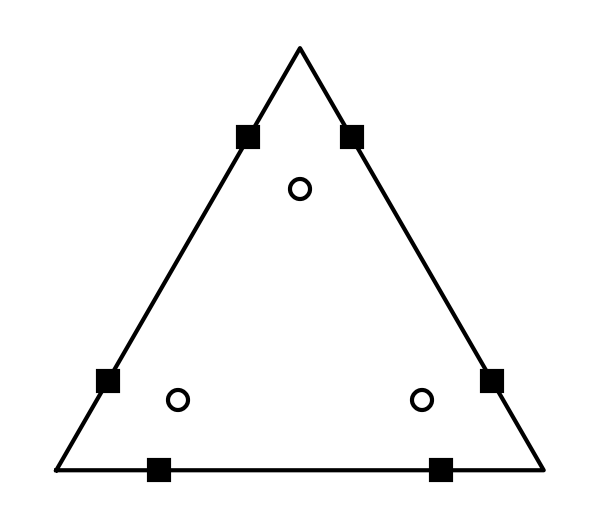
\includegraphics[width=0.16\textwidth]{figures/p1_Omega}\\
            3 nodes\end{center}} & 
        \parbox[b]{0.2\textwidth}{%
            \begin{center}%
                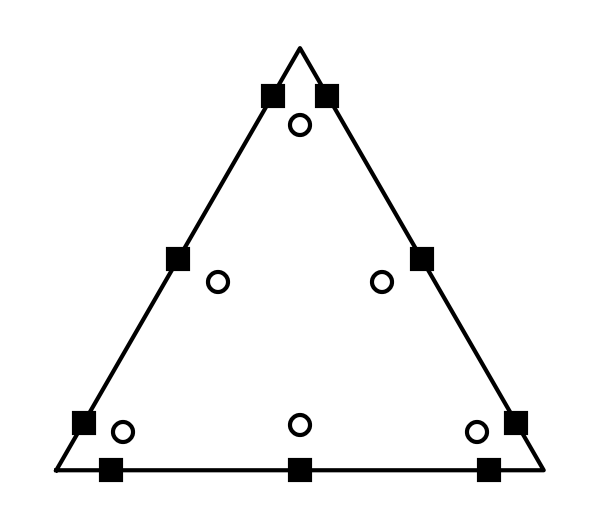
\includegraphics[width=0.16\textwidth]{figures/p2_Omega}\\
                6 nodes\end{center}} &
            \parbox[b]{0.2\textwidth}{%
                \begin{center}%
                    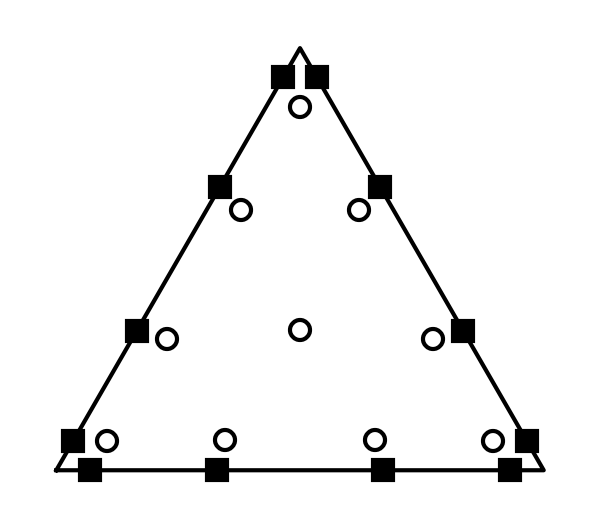
\includegraphics[width=0.16\textwidth]{figures/p3_Omega}\\
                    10 nodes\end{center}} &
                \parbox[b]{0.2\textwidth}{%
                    \begin{center}%
                        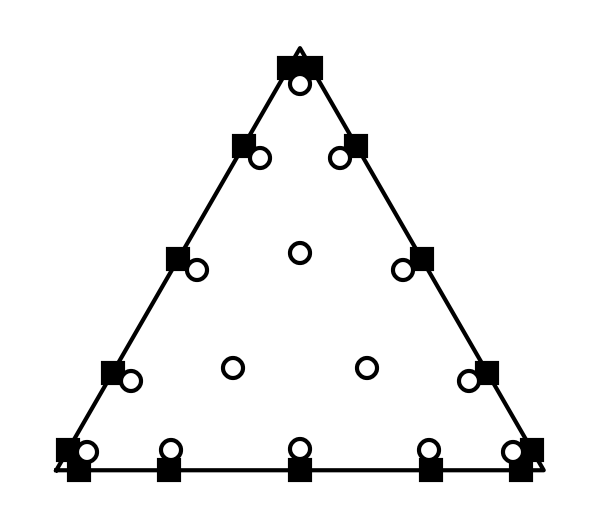
\includegraphics[width=0.16\textwidth]{figures/p4_Omega}\\
                        15 nodes\end{center}} \\\hline
                \vspace*{-0.12\textwidth}\textbf{SBP}-$\bm{\Gamma}$ & 
                \parbox[b]{0.2\textwidth}{%
                    \begin{center}%
                        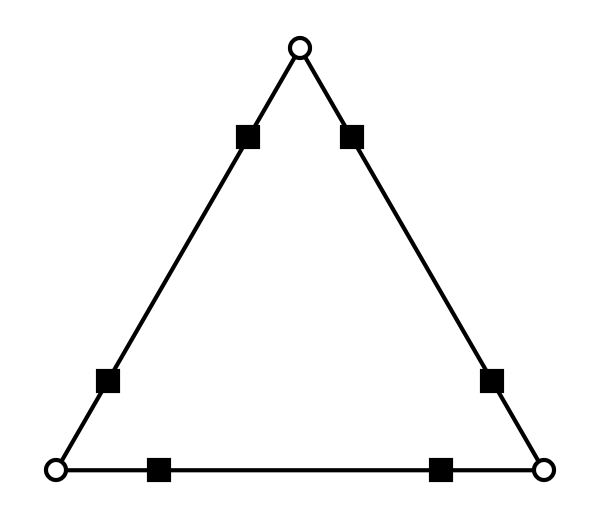
\includegraphics[width=0.16\textwidth]{figures/p1_Gamma}\\
                        3 nodes\end{center}} &
                \parbox[b]{0.2\textwidth}{%
                    \begin{center}%
                        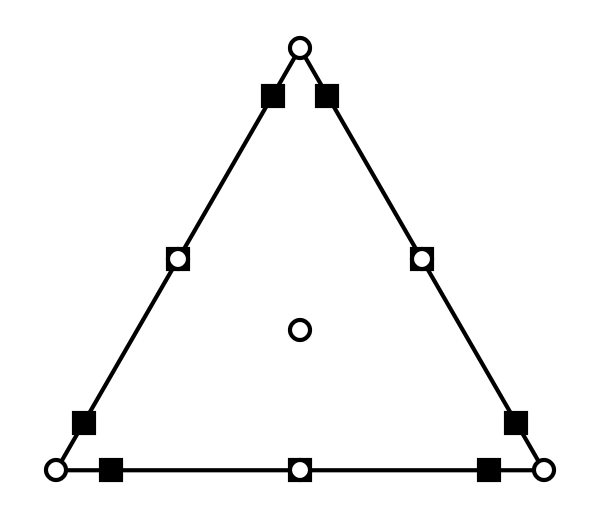
\includegraphics[width=0.16\textwidth]{figures/p2_Gamma}\\
                        7 nodes\end{center}} &
                \parbox[b]{0.2\textwidth}{%
                    \begin{center}%
                        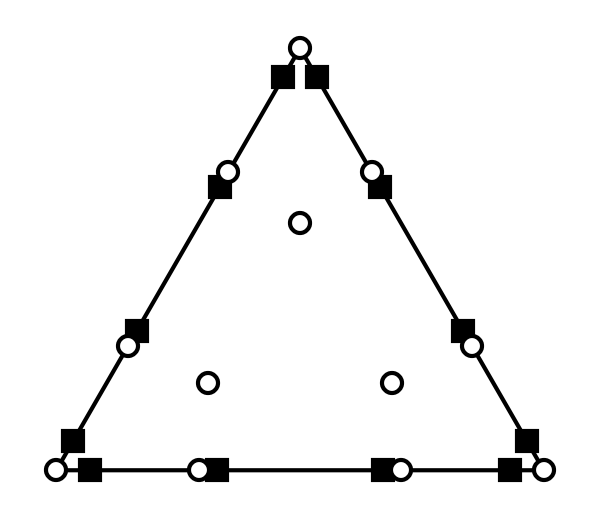
\includegraphics[width=0.16\textwidth]{figures/p3_Gamma}\\
                        12 nodes\end{center}} &
                \parbox[b]{0.2\textwidth}{%
                    \begin{center}%
                        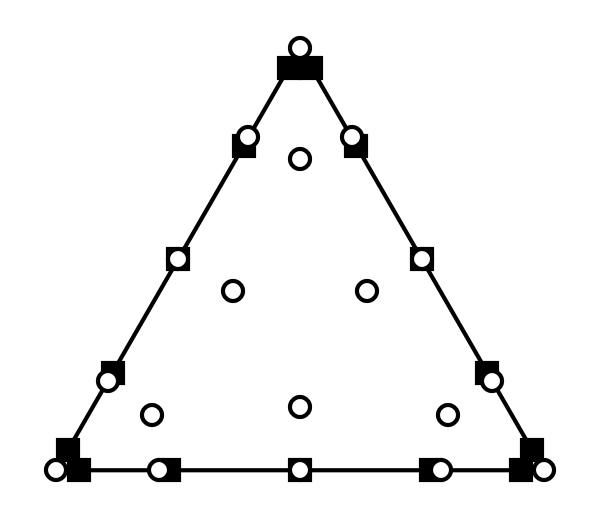
\includegraphics[width=0.16\textwidth]{figures/p4_Gamma}\\
                        18 nodes\end{center}} \\\hline
            \end{tabular}
\end{alertblock}
\vskip-0.6cm
\begin{alertblock}{The expected convergence rates and stability properties 
        
        were obtained}       
\begin{itemize}
    \item \textbf{Convergence rates of solution and functional}
    \begin{figure}  
        \centering
        \begin{subfigure}[b]{0.48\linewidth}
            \centering
            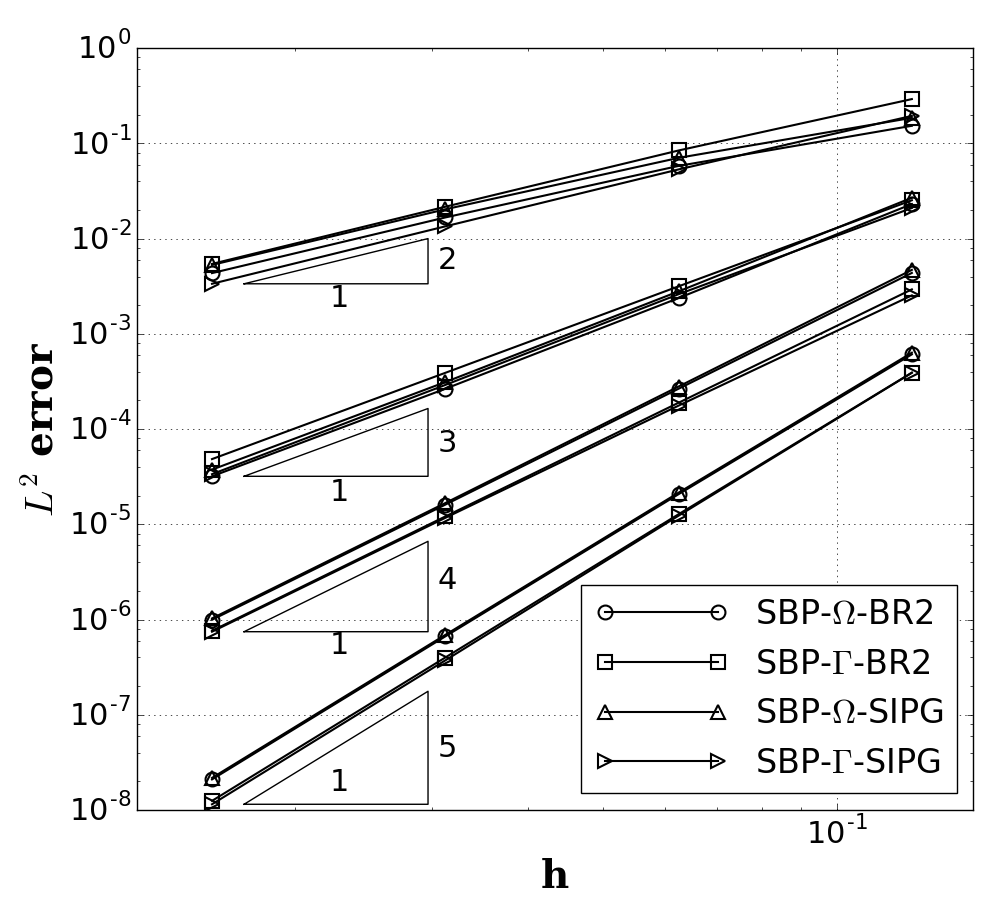
\includegraphics[width=1.\linewidth]{figures/p_accuracy.png}
             \subcaption*{Solution accuracy, $O(p+1)$}
%            \label{fig:p_accuracy}
        \end{subfigure}%
        \begin{subfigure}[b]{0.48\linewidth}
            \centering
            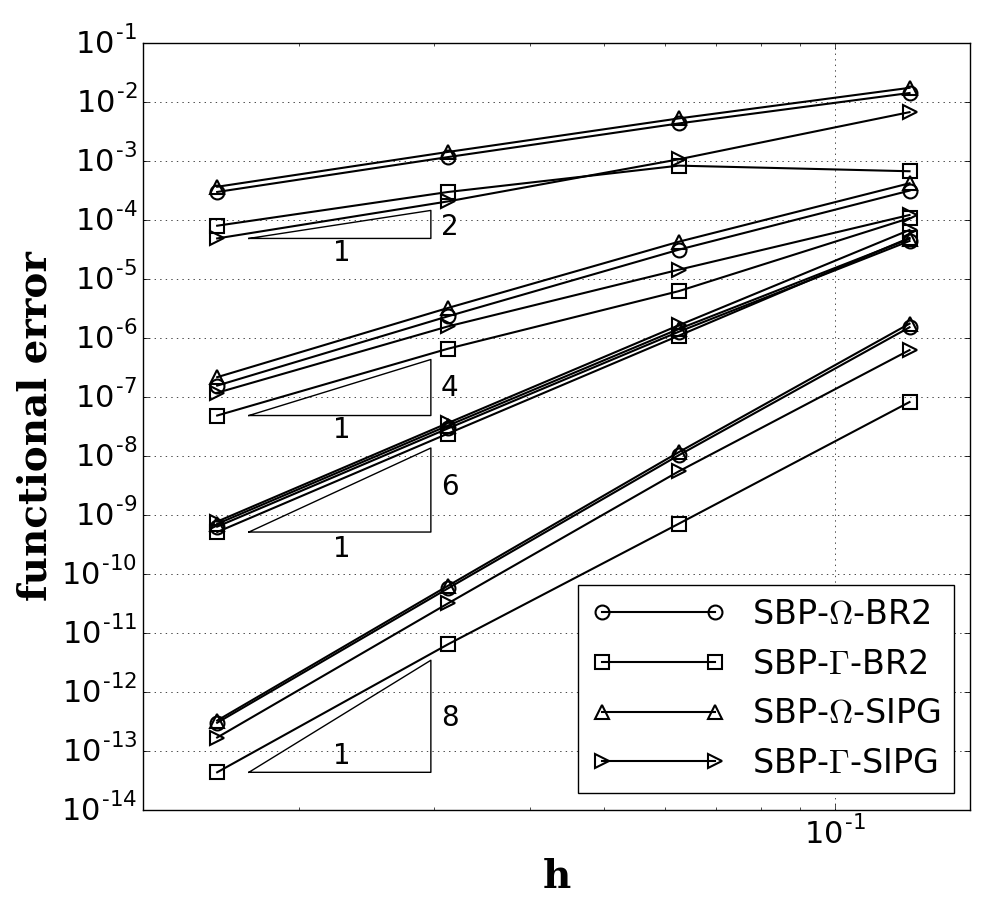
\includegraphics[width=1.\linewidth]{figures/j_accuracy.png}
             \subcaption*{Functional accuracy, $O(2p)$}
%            \label{fig:j_accuracy}
        \end{subfigure}
%        \caption{Convergence rate study }
    \end{figure}
%        \item
%        \textbf{Tightness of stability bound:} We scale $\Sig^{(1)}$ and $\Sig^{\fnc{D}}$ by a relaxation factor $\alpha$, 
%        which serves as a measure of tightness of the stability bound, i.e.,
%          
%        \begin{itemize}
%            \item overly conservative SAT penalties will allow for $\alpha \ll 1$; 
%            \item necessary and sufficient stability condition only permit $\alpha \ge 1$.
%        \end{itemize}
%        \normalfont
%        \begin{figure} 
%            \begin{subfigure}{0.45\textwidth}
%                \centering
%                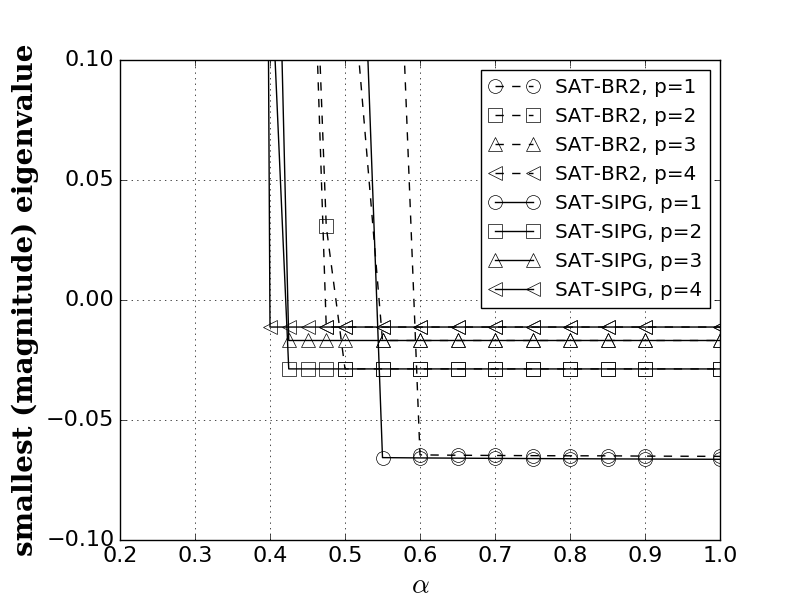
\includegraphics[width=1.0\linewidth]{figures/relaxation_eigMin_gamma.png}
%%                \subcaption{SBP-$\Gamma$}
%                \label{fig:relaxation_cn_gamma}
%            \end{subfigure}
%            \begin{subfigure}{0.45\textwidth}
%                \centering
%                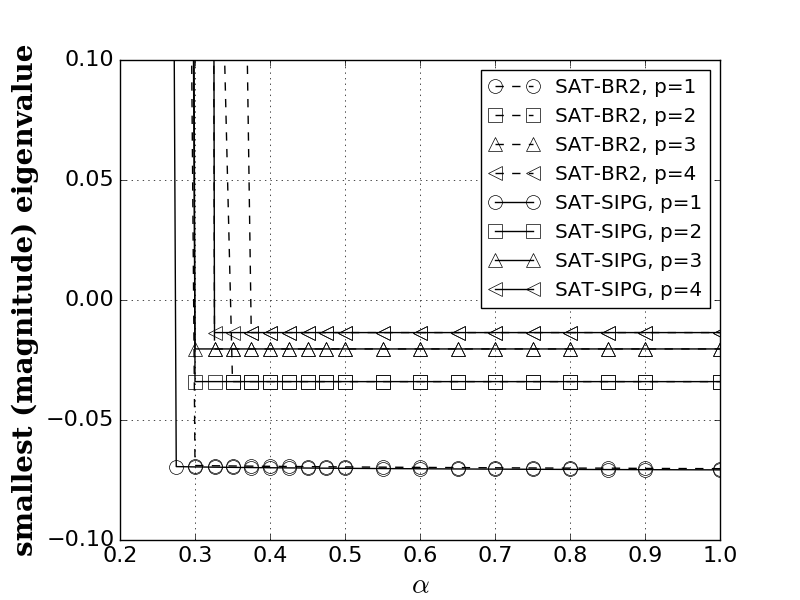
\includegraphics[width=1.0\linewidth]{figures/relaxation_eigMin_omega.png}
%%                \subcaption{SBP-$\Omega$}
%                \label{fig:relaxation_cn_omega}
%            \end{subfigure} 
%            \caption{Relaxation effect on SATs, left:SBP-$\Gamma$, right:SBP-$\Omega$}
%            \label{fig:relaxation}   
%        \end{figure}
    
%    \begin{minipage}{0.25\linewidth}

    \begin{columns}[t] 
    \begin{column}{0.3\textwidth}
        \item \textbf{Energy stability:}
        
        If the penalty matrices do not satisfy the requirements of the stability theory, the solution norm may grow exponentially.
    \end{column}
%        \setbeamertemplate{caption}{default}
    \begin{column}{0.625\textwidth}
        \begin{figure} 
            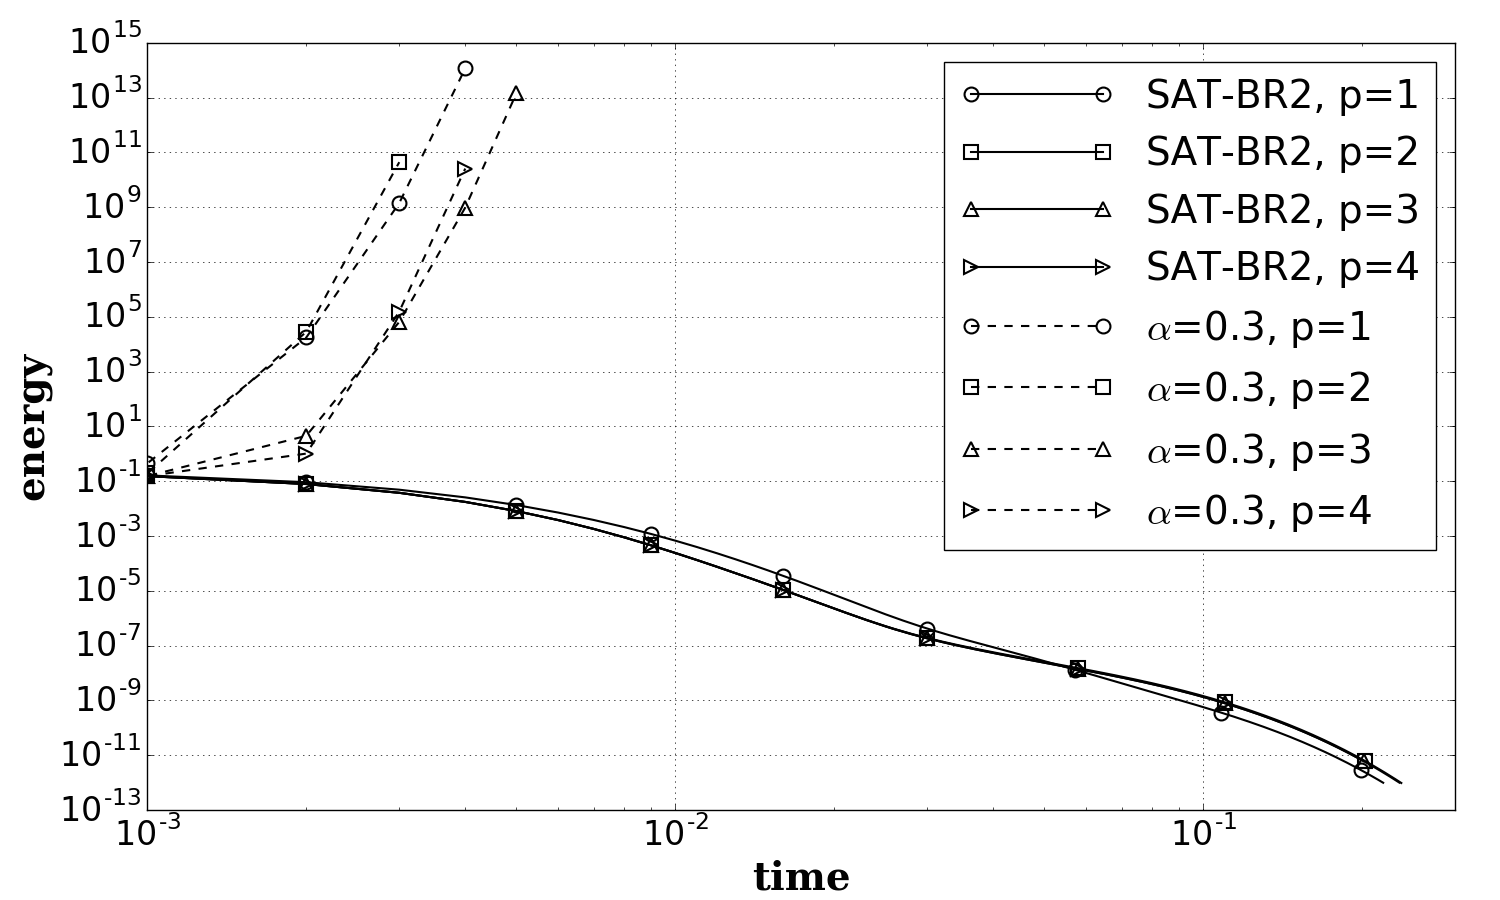
\includegraphics[width=0.92\linewidth]{figures/energy_stability.png}
            \caption*{Energy history of homogeneous problem using BDF2 and SBP-$\Gamma$}
        \end{figure}
    \end{column}
%\vskip-0.25cm
\end{columns}
\end{itemize}

%     \end{itemize}
\end{alertblock}
    %----------------------------------------------------------------------------------------
    %	REFERENCES
    %----------------------------------------------------------------------------------------
    
%    \begin{block}{References}
%        
%        \nocite{*} % Insert publications even if they are not cited in the poster
%        \footnotesize{\bibliographystyle{unsrt}
%            \bibliography{sample}\vspace{0.15in}}
%        
%    \end{block}
    
    %----------------------------------------------------------------------------------------
    %	ACKNOWLEDGEMENTS
    %----------------------------------------------------------------------------------------
    
%    \setbeamercolor{block title}{fg=red,bg=white} % Change the block title color
%    
%    \begin{block}{Acknowledgements}   
%        \footnotesize{\rmfamily{J. Hicken was partially funded by the Air Force Office of Scientific Research Award FA9550-15-1-0242. The authors gratefully acknowledge this support. We also thank RPI's Scientific Computation
%                Research Center for the use of computer facilities.}} \\
%        
%    \end{block}
    
    %----------------------------------------------------------------------------------------
    %	CONTACT INFORMATION
    %----------------------------------------------------------------------------------------
    
    %\setbeamercolor{block alerted title}{fg=black,bg=norange} % Change the alert block title colors
    %\setbeamercolor{block alerted body}{fg=black,bg=white} % Change the alert block body colors
    %
    %\begin{block}{Contact Information}
    %
    %\begin{itemize}
    %\item Web: \href{http://www.university.edu/smithlab}{http://www.university.edu/smithlab}
    %\item Email: \href{mailto:john@smith.com}{john@smith.com}
    %\item Phone: +1 (000) 111 1111
    %\end{itemize}
    %
    %\end{block}
    %
    %\begin{center}
    %\begin{tabular}{ccc}
    %\includegraphics[width=0.4\linewidth]{logo.png} & \hfill & \includegraphics[width=0.4\linewidth]{logo.png}
    %\end{tabular}
    %\end{center}
    
    %----------------------------------------------------------------------------------------
\end{column}
\begin{column}{\sepwid}\end{column} % Empty spacer column
\begin{column}{\sepwid}\end{column} % Empty spacer column

\end{columns} % End of all the columns in the poster

\end{frame} % End of the enclosing frame

\end{document}
